% Human civilisation has used microbes and cell cultures since at least the Neolithic for fermentation \cite{liu2018fermented}. 
After the introduction of recombinant protein production in 1977 \cite{itakura1977expression}, a large number of monoclonal antibodies, hormones, enzymes and other proteins of pharmaceutical, industrial and scientific importance are being synthesised using microbes such as bacteria and yeast, insect cells and mammalian cells. Consequently, recombinant proteins currently has a market value in billions of dollars, making it one of the highly valued technologies \cite{walsh2014biopharmaceutical, puetz2019recombinant}. 


There has been much research to improve the recombinant protein production technology. In particular, the development of the pET vector system in 1991 has revolutionised the use of \textit{Escherichia coli} for protein production \cite{dubendorf1991controlling}. \textit{E. coli} is often the host of choice because it is relatively inexpensive, and has a faster growth rate than other expression hosts \cite{Rosano2014-oq, demain2009production}. Now there are a multitude of optimised vectors such as pGEX, pMAL and pET as well as a number of engineered strains of \textit{E. coli} such as BL21 and BL21(D3). Several guidelines and practices have also been proposed to maximise the chances of successful experiments \cite{Berlec2013-mb, Rosano2014-oq}. Furthermore, several high-throughput methods have made the process scalable \cite{stevens2000design, braun2003high, jia2016high}. These new advancements has made the process of recombinant protein production much easier and economical. 


\section{Recombinant protein production}
The initial step in recombinant protein production is a successful protein expression. The expressed protein then needs to be soluble for use in many structural, functional and pharmaceutical studies where concentrated protein samples are desired \cite{Kramer2012-wk, Hou2018-yd}. Despite almost 40 years of refinements in protocols and technology, around half of the recombinant protein expression experiments fail at the expression stage and nearly half of expressed protein are insoluble \cite{targetdbmetrices} (Figure \ref{fig:fail_succ}). This makes the protein production process more challenging. Predicting protein expression and solubility can help plan the experiment and save time and resources. Furthermore, using a highly optimised target gene can increase the success rate of recombinant protein production.


\begin{figure}[htbp!]
\center
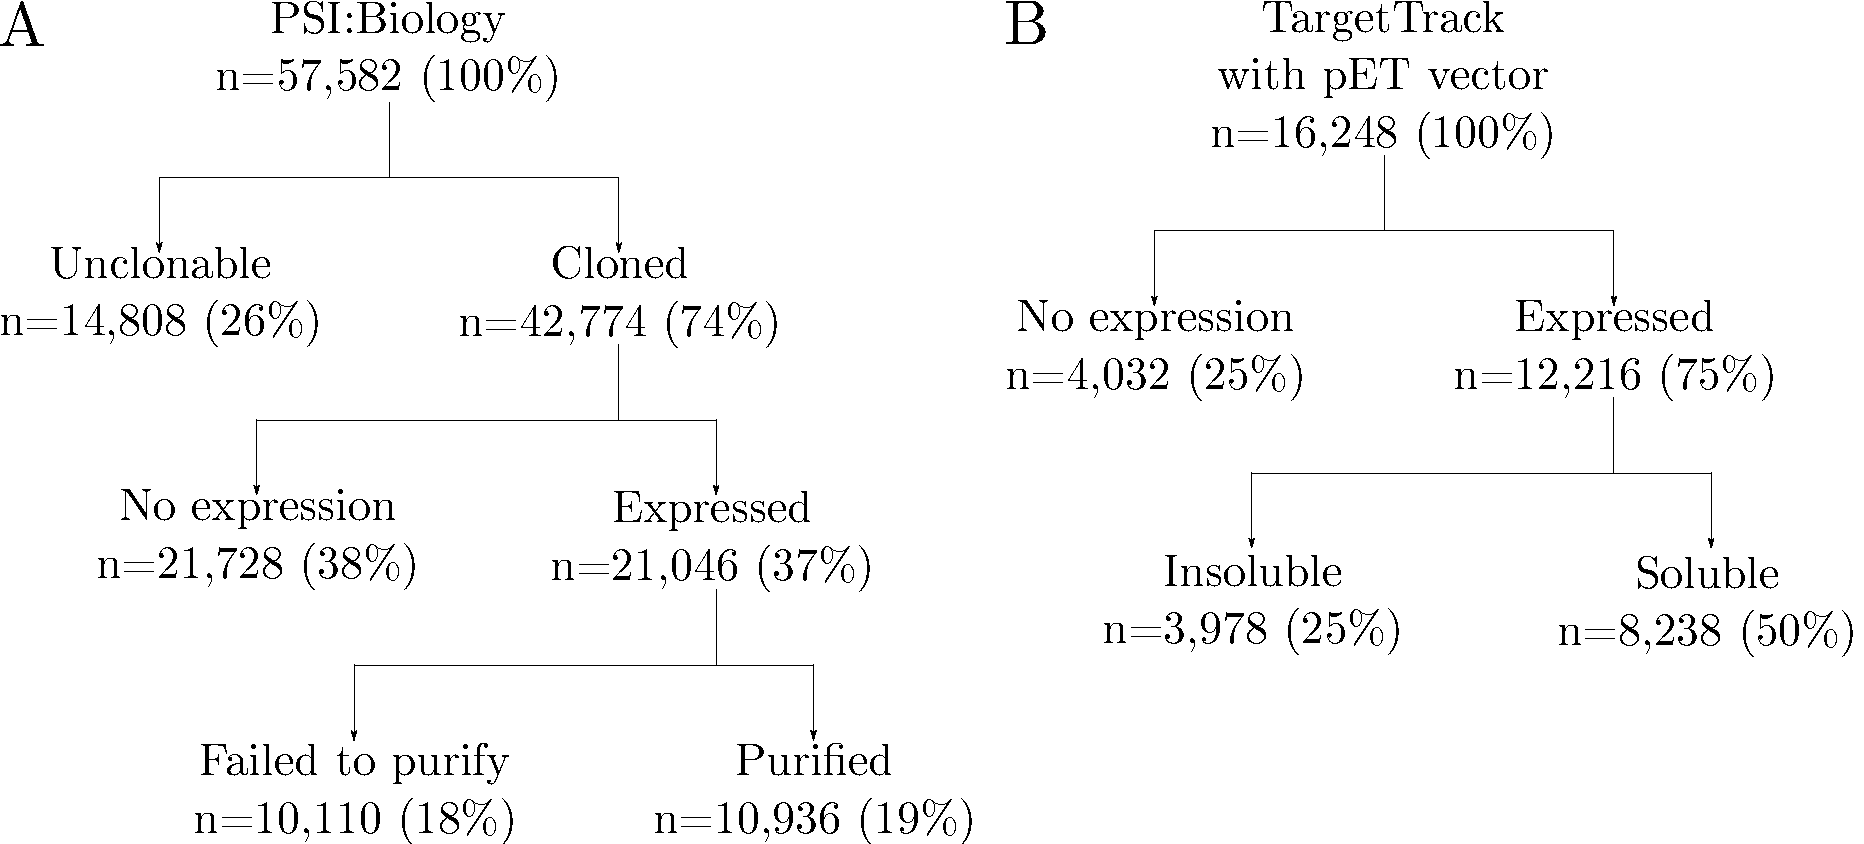
\includegraphics[width=1\textwidth]{chapters/Introduction/Figures/Status_of_protein_expression(2).pdf}
\caption[The success rate of recombinant protein production is around a quarter.]{\textbf{The success rate of recombinant protein production is around a quarter. (A)} All experiments, using different vectors and hosts, preformed for deposition to the TargetTrack database shows around $19\%$ of experiments are purified. Data taken from Protein Structural Initiative (PSI:Biology) metrics. \textbf{(B)} A subset of experiments from TargetTrack database using pET vector and \textit{E. coli} as expression host, shows $50\%$ of experiments produce soluble proteins. }%the List of Figures because of the *}
\label{fig:fail_succ}
\end{figure}


In the following sub-sections, we will discuss these two steps\textemdash protein expression and solubility in details. Unless otherwise stated, these discussions will refer to prokaryotes, in particular, \textit{E. coli} based systems. 

% Protein expression
\subsection{Protein expression}
Protein expression is the process by which protein is synthesised using the information in the messenger RNA (mRNA) (Figure \ref{fig:tranc_transl}). 


\begin{figure}[htbp!]
\center
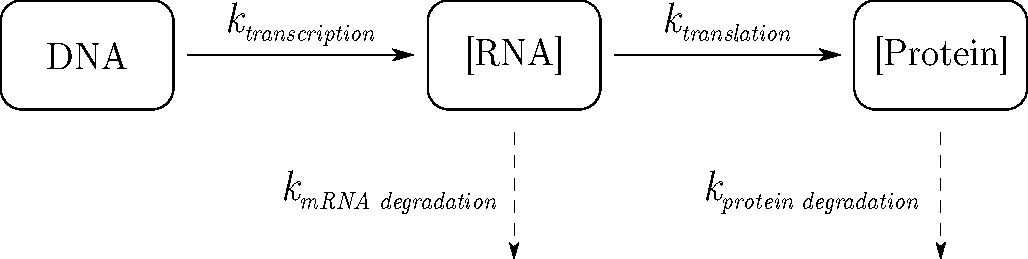
\includegraphics[width=0.7\textwidth]{chapters/Introduction/Figures/transc_transl.pdf}
\caption[Protein expression depends on the rates of RNA and protein synthesis and their degradation.]{\textbf{Protein expression depends on the rates of RNA and protein synthesis and their degradation.} Solid arrow represents synthesis whereas dashed arrow represents degradation. [RNA], concentration of mRNA; [Protein], concentration of protein; $k_{transcription}$, rate of transcription; $k_{translation}$, rate of translation; $k_{mRNA\ degradation}$, rate of mRNA degradation; $k_{protein\ degradation}$, rate of protein degradation. Figure redrawn from Abreu \textit{et al.} (2009).}%the List of Figures because of the *}
\label{fig:tranc_transl}
\end{figure}

Intuitively, we expect the protein yield to be predictable using mRNA levels, the correlation is lower than expected \cite{Abreu2009-zf, Taniguchi2010-uq, Bernstein2002-gg}. This reflects the complexities of the underlying process. The amount of protein produced is determined by translation rate and protein degradation (Figure \ref{fig:tranc_transl}).  This dynamic system can be mathematically described by a first order differential equation \cite{Abreu2009-zf} whose solution at equilibrium gives the following relationship relationship between protein concentration $(P_{\infty})$, mRNA concentration $(R_{\infty})$, translation rate $(k_{translation})$ and protein degradation rate $(k_{protein\ degradation})$ :

\begin{equation}
    \frac{P_{\infty}}{R_\infty} = \frac{k_{translation}}{k_{protein\ degradation}}
\end{equation}

There are various mechanisms regulating translation and protein degradation, so the correlation between $(P_{\infty})$ and $(R_{\infty})$ is not perfect. Squared Pearson's correlation is around $0.4$ for many organisms \cite{Abreu2009-zf}. Assuming the protein degradation rate $(k_{protein\ degradation})$ to be a constant, the ratio of $P/R$ depends upon the translation rate $(k_{translation})$ only. Hence, the amount of protein can be modulated by tuning  $k_{translation}$.

\subsection{Translation}

Translation in prokaryotes is \textit{initiated} when the small ribosome subunit $30S$ binds to the Shine-Dalgarno sequence and moves upto the start codon. The currently accepted model is that the initiator tRNA charged with N-formylmethionine, initiation factor (IF-2) and guanosine triphosphate (GTP) binds with this subunit followed by the release of IF-3 \cite{hames2005biochemistry}. This complex is called the 30S initiation complex. IF-1 and IF-2 are released and the large ribosomal subunit $50S$ now binds followed by the hydrolysis of GTP, to form a $70S$ initiation complex. 

After the formation of initiation complex, the decoding of information in the mRNA begins. This is called \textit{translation elongation}. The $70S$ complex consists of three active sites: peptidyl-tRNA site (P site), aminoacyl-tRNA site (A site) and exit site (E site). Initially, the start codon and the successive codon of mRNA is positioned at P site and A site respectively. The initiator tRNA charged with N-formylmethionine is coupled with start codon at the P site and the corresponding aminoacyl-tRNA is coupled to the next codon at the A site through codon-anticodon pairing (Figure \ref{fig:prokaryotic_translation}). Peptide bond is formed between the amino acid carried by tRNA at P and A site to give a dipeptide. tRNA at P site is translocated to E site, tRNA at A site to P site and the ribosome moves along the mRNA. The deactylated tRNA at E site is released. Since the A site is now empty, it receives the next aminoacyl-tRNA and the process continues adding an amino acid to C terminal of the dipeptide. 


Once the ribosome encounters a stop codon, release factor (RF1 or RF2 and RF3) bind to the ribosome resulting in a tranfer of polypeptide to a water molecule rather than aminoacyl-tRNA. The free polypeptide is released from the ribosome and $70S$ ribosome disassociates into $30S$ and $50S$ subunits. This step is called \textit{translation termination}. 

%%TODO - FIGURE FOR TRANSLATION


\begin{figure}[!hbtp]
    \centering
    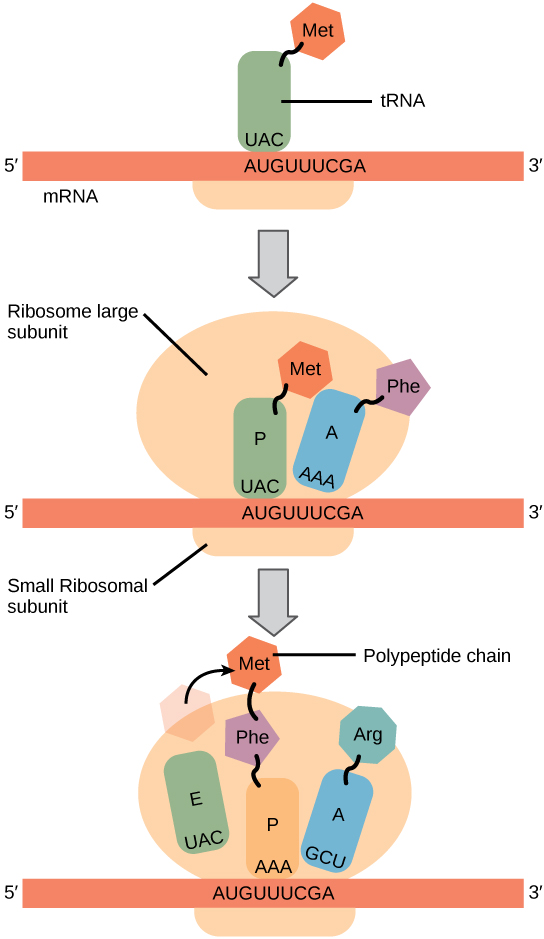
\includegraphics{chapters/Introduction/Figures/translation.jpg}
    \caption[Prokaryotic translation.]{\textbf{Prokaryotic translation.} Initiator tRNA binds to the smaller subunit at the start codon. Larger subunit joins to form a translation initiation complex such that initiator tRNA is at P site and the next aminoacyl-tRNA is at A site. Initiator tRNA moves to the E site, dipeptide is formed at the P site and new aminoacyl-tRNA is received at the A site. Figure from OpenStax College, Concepts of Biology. OpenStax CNX (Creative Commons license: CC BY 4.0) }%the List of Figures because of the *}
    \label{fig:prokaryotic_translation}
\end{figure}


\subsection{mRNA features and their roles in translation}
Translation rate depends on the rate formation of translation initiation complex and utilisation of available tRNA pool. Several features of a mRNA sequence are suggested to explain these two major dependencies of translation rate. However, many mRNA features are not independent, making it hard to distinguish the impacts of individual features \cite{mauger2019mrna}. The features can be classified into three categories: codon preferences, mRNA folding (secondary structure) and mRNA:ncRNA avoidance. These three categories of features is the basis to understand and optimise protein production. Hence, we will describe them in more details:

% mRNA features
%Codon Analysis


\subsubsection{Features based on codon analysis}
This category measures the bias in codon usage relative  to endogenous mRNAs. Higher values of these indices is an indicator that the given mRNA sequence follows the codon usage pattern of the host. Features under this category are the codon adaptation index (CAI) \cite{Sharp1987-ed}, tRNA adaptation index (tAI) \cite{ Reis2004-dl, Sabi2014-je} and related metrics such as codon pair usage \cite{Gutman1989-pn}. For example: the codon adaptation index (CAI) for a given protein is the harmonic mean of the relative adaptiveness $w$ \cite{Sharp1987-ed} of the codons:

\begin{equation}
    CAI_{g}=(\prod_{i=1}^{N} w_i)^{1/N}
    \label{eqn:cai}
\end{equation}
where $w_i$ is the relative adaptiveness of the $i^{th}$ codon which is the ratio of observed frequency of the codon $f_i$ upon consideration to the frequency of the most frequent synonymous codon. $$w_i = \frac{f_i}{max(f_i)}$$ 

Based upon the idea of CAI, tAI was developed to measure the translational efficiency by taking into account of tRNA concentration and codon-anticodon coupling efficiency. We first define the absolute adaptiveness $W_i$ of codon $i$ as:

\begin{equation}
    W_i = \sum_{j=1}^{n_i} (1 - s_{ij})tGCN_{ij}
\end{equation}
where $n_i$ is the number of anticodons pairing with codon $i$, $tGCN_{ij}$ is the copy number of the $j^{th}$ tRNA that recognizes the $i^{th}$ codon. $tGCN_{ij}$ is correlated with the tRNA concentration \cite{kanaya1999studies, novoa2012role}. $s_{ij}$ is a constraint on the codon-anticodon pairing and has values between $0$ (more efficient pairing) and $1$ (less efficient pairing). The relative adaptiveness $w_i$ of the $i^{th}$ codon is  $W_i$ normalised by maximum of $W_i$ among all codons. If $W_i$ is zero, then the relative adaptiveness is the mean of all $W_i$. Once $w_i$ are found, the tAI is the harmonic mean as in Equation \ref{eqn:cai}. 


Both CAI and tAI measures are equivalent to a zeroth order Markov model whereas codon pair usage or di-codon frequency is essentially a first order Markov model. It is thought that a higher value of these indices means that the sequence can utilise the available tRNA pool more efficiently which causes an increase in efficiency of translation \cite{ikemura1985codon, Gutman1989-pn, Sharp1987-ed, Reis2004-dl, Sabi2014-je, Brule2017-mx}. However, this proposition has been challenged and studies suggest that mRNA secondary structure might be more important in explaining translation efficiency.  \cite{Kudla2009-tl, Boel2016-jd, Cambray2018-kn}.

%% Secondary structure
\subsubsection{Secondary structure}
%Translation initiation in prokaryotes begins after the ribosomal $30S$ subunit binds to the Shine-Dalgarno sequence and recognises the start codon. The larger subunit is then assembled to form a translation initiation complex, which moves along the transcript, decoding the codons to form a polypeptide chain. However, if this 
If the region around a translation initiation site forms a strong secondary structure, this leads to disruption of the formation of initiation complex, which inhibits translation (Figure \ref{fig:sec_str_rbs}) \cite{Kudla2009-tl, Espah_Borujeni2014-vy, Tuller2015-ts}. Recent studies show that the RNA structure stability of this region explains variation in protein expression better then codon usage \cite{Kudla2009-tl, Plotkin2011-ak, Cambray2018-kn} indicating that translation initiation is a rate limiting step for translation. Furthermore, secondary structure has been shown to change the functional half-life of mRNA and thus further influence protein expression \cite{mauger2019mrna}. Minimum free energy (MFE) of mRNA is widely used to measure the strength and stability of secondary structure. A way to find the MFE is to enumerate all possible structures of a given mRNA and then find the minimum. However, this is impractical because combinatorial explosion occurs quickly as the length of mRNA increases. Clever dynamic programming algorithms has made this problem tractable the details of which is described below.


\begin{figure}[htbp!]
\center
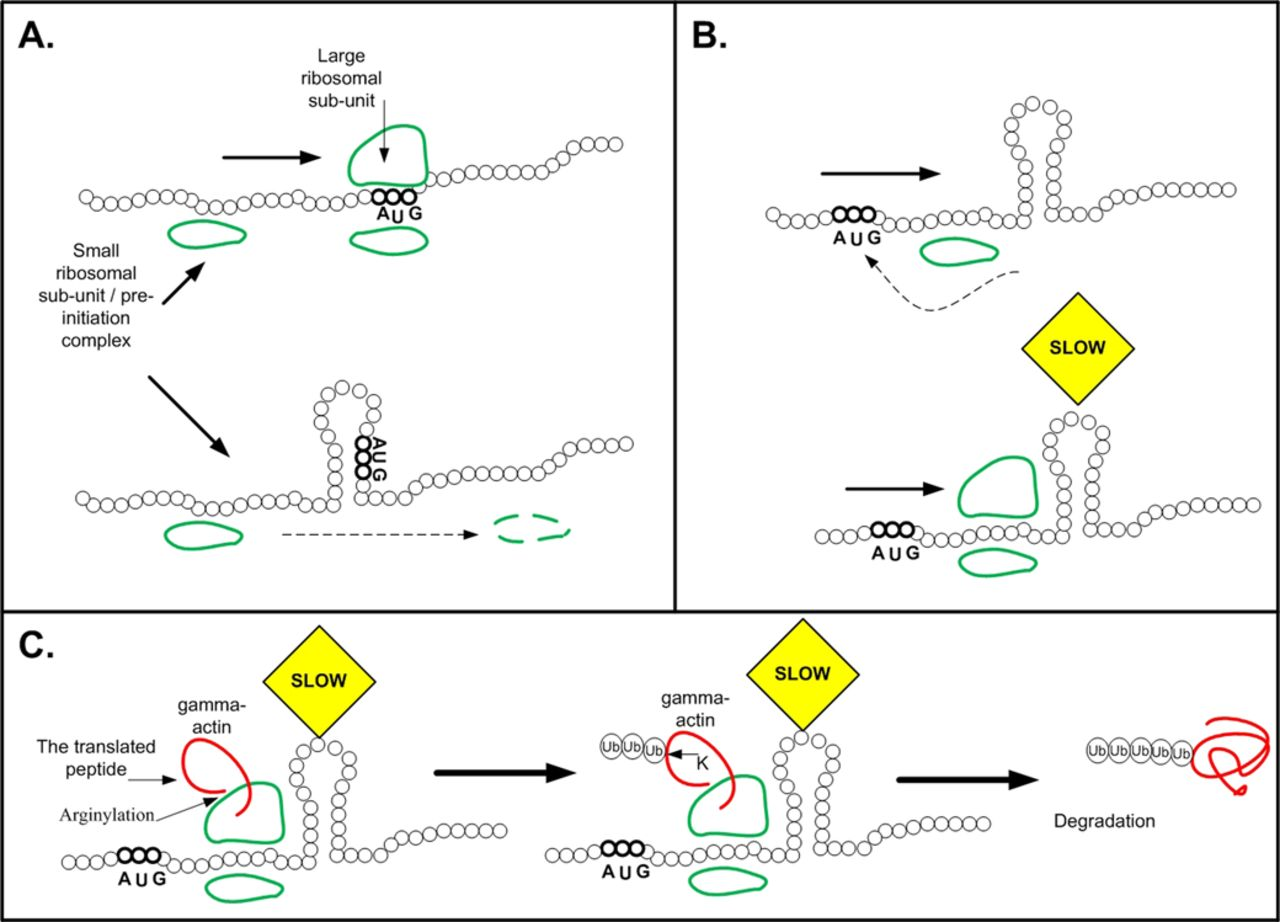
\includegraphics[width=1\textwidth]{chapters/Introduction/Figures/sec_str_rbs.jpg}
\caption[Secondary structure at the translation initiation site inhibits translation.]{\textbf{Secondary structure at the translation initiation site inhibits translation. (A) } The start codon AUG is recognised by the pre-initiation complex if the secondary structure is weak (top) but fails to do so in presence of a strong structure (bottom). \textbf{(B)} Presence of strong structure downstream of translation initiation site prevents the movement of pre-initiation complex (top) which could improve translation efficiency by improving ribosomal allocation (bottom). \textbf{(C)} Such downstream structures could influence post-translation modification by slowing down the ribosome. For example: lysin residues in arginylated gamma actin are exposed due to slow translation and undergo ubiquitination. Figure from Tuller and Zur, (2011) (Creative Commons license: CC BY ) }%the List of Figures because of the *}
\label{fig:sec_str_rbs}
\end{figure}



\paragraph{Computation of minimum free energy (MFE) and suboptimal structures}
Thermodynamically, an RNA structure with the lowest Gibb's free energy is the most stable. This energy is called minimum free energy. Thermodynamic ensembles usually follow the principle of locality, which says that interactions occur only between neighbouring particles. For example: In the Ising model of magnetism, spin interactions happen only between the nearest particles. Similarly, MFE is also calculated by using so called 'Turner parameters' \cite{turner2009nndb} in a nearest neighbouring model and a set of recursive equations called Zuker's algorithm \cite{zuker1981optimal}. However, the accuracy of the computed MFE is only within $5-10\%$ and a large number of alternate RNA structures lie within $5-10\%$ of the predicted global minimum \cite{eddy2004rna}. This prompts us to calculate some other free energies for different suboptimal conformations that RNA may achieve in a near thermodynamic equilibrium. Furthermore, depending on the criteria to pick an \textit{optimal} sturcture from a Boltzmann's ensemble, suboptimal structures may not lie near the thermodynamic equilibrium at all. For example: Ding \textit{et al.} \cite{ding2005rna}  found that structures tend to form clusters in a Boltzmann's ensemble. Instead of free energy, if we use these clusters as a criteria for sampling, then structure that has a minimum distance from all clusters is the optimial structure \cite{lorenz2016predicting}. This structure is also known as centroid structure and other structures around the centroid may as well be regarded as suboptimal.



There were some early attempts to compute suboptimal structures for example, by Zuker \cite{zuker1989finding} and Waterman \textit{et al.} \cite{waterman1985dynamic}. However, the backtracing procedure in their algorithms was not efficient enough to compute energies for longer RNA molecules. This problem was solved by McCaskill \cite{mccaskill1990equilibrium} by proposing an efficient algorithm to compute energy through a partition function which has the same time complexity as Zuker's algorithm for MFE $(\mathcal{O}(n^{3}))$.

\paragraph{Partition function and base pairing probabilities}
Consider a structure $s$ of an RNA molecule with free energy $E(s)$. In a thermodynamic ensemble of different structures at equilibrium, using the principle of maximum entropy, we see that the probability that the given RNA has the structure $s$ follows a Boltzmann distribution:

\begin{equation}
    p(s) \propto e^{-\beta E(s)}
\end{equation}

where $\beta$ is called 'thermodynamic beta' and equals $1/k_B T$, where $k_B$ is the Boltzmann's constant and $T$ is the absolute temperature (Subsection \ref{subsection:sim_anneal} Simulated annealing ). Since sum of probabilities over set of all structures $\Xi$, must be equal to unity, we have:

\begin{equation}
\begin{aligned}
    \sum_s p(s) &= \frac{1}{Z} \sum_{s\in\Xi} e^{-\beta E(s)}  = 1  \\
    Z &= \sum_{s\in\Xi} e^{-\beta E(s)} 
\end{aligned}
\label{eqn:part_func}
\end{equation}

The quantity $Z$, which plays a role of normalisation of probabilities, is called the \textit{canonical partition function}. Many thermodynamic parameters of interest can be derived from $Z$, for example, free energy $G$ of RNA in terms of $Z$ is given by:

\begin{equation}
\label{eqn:free_en}
    G = -\frac{1}{\beta} \ln(Z)
\end{equation}

The efficient dynamic programming to enumerate $Z$ was proposed by McCaskill \cite{mccaskill1990equilibrium} with time complexity of $\mathcal{O}(n^{3})$. This method is essentially a recursive decomposition of $Z$ similar to Zuker's algorithm only difference being the addition in Zuker's relation are now substituted by product because free energies are additive. If $E$ is the total free energy and $E_L$ are the energy contributions from various types of loops (hairpin, stacked pair, bulges, interior loops, multiloops) in a structure, then:

\begin{equation}
    E = \sum_L E_L
    \label{eqn:free_en_add}
\end{equation}

If we suppose the term $Q_{ij}^b$ accounts for all loops $L$ enclosed by $i,j$, we see that additivity of free energy (Equation \ref{eqn:free_en_add}) implies a multiplicative contribution to the partition function (\ref{eqn:part_func}) which gives the following recursive equation :

\begin{equation}
    Q_{ij}^b = \sum_L e^{-\beta E_L} \prod_{i<h<k<j} Q_{hk}^b
    \label{eqn:mcc_restr_part}
\end{equation}

Using this restricted partition function term for loop contributions, the total partition function between $i^{th}$ and $j^{th}$ nucleotides ($Q_{ij}$) can now be written as:

\begin{equation}
    Q_{ij} = Q_{i j-1} + \sum_{i \leq k <j} Q_{i k-1} Q_{kj}^b
    %where, by convention, Q_{i, i} = Q_{i, i-1} = 1.
    \label{eqn:mcc_full}
\end{equation}

The full partition function of RNA with $N$ nucleotides is given by $Z = Q_{1N}$. Equations \ref{eqn:mcc_restr_part} and \ref{eqn:mcc_full} are McCaskill's recursions for partition function. Once $Z$ is known, the probability of any structure $s$ with free energy $E(s)$ is given by:

\begin{equation}
\label{eqn:prob_part_func}
    p(s) = \frac{1}{Z} e^{-\beta E(s)}
\end{equation}

The computational approach outlined above is very generic and can be used for other specific cases. For example: if we want to know the probability that $[i^{th}, j^{th}]$ nucleotides are paired, then we can modify Equation \ref{eqn:part_func}, where partition function is found by simply summing Boltzmann's factor over all structures $\zeta$ where $[i^{th}, j^{th}]$ nucleotides are paired ($\zeta \subseteq \Xi$, where $\Xi$ is the ensemble of structures):

\begin{equation}
    Z_p = \sum_{s\in\zeta} e^{-\beta E(s)}
\end{equation}

The base pairing probabilities are, given by equation \ref{eqn:prob_part_func} with an appropriately computed $Z$. % which is Z on the above equation.


%% Avoidance
\subsubsection{mRNA:ncRNA avoidance}
Recently, Umu et al \cite{Umu2016-zq} found that in bacteria and the archaea, the strength of interactions between mRNAs and non-coding RNAs (ncRNAs) anti-correlate with protein levels. These signals are particularly obvious at the translation initiation site, suggesting that there is an avoidance of inappropriate interactions for highly expressed proteins. However, from a large pool of mRNA and ncRNA, a complete avoidance of interactions is unlikely and a trade off exists between interactions and protein expression. Further, it is suggested that compartmentalisation should minimise these cross talk interactions in eukaryotes. Compartmentalisation has been a topic of considerable research and is linked with noise filtering in gene expression and cellular feedback process \cite{rao2002control, stoeger2016passive, banani2017biomolecular, dong2017shaping}. We now outline in brief, the necessary background to understand the computation of RNA interactions and mRNA:ncRNA avoidance.


\paragraph{Unpairing of bases and accessibility}
McCaskill’s equations \ref{eqn:mcc_restr_part} and \ref{eqn:mcc_full} for the partition function can also be `inverted' to find the probability that $[i^{th}, j^{th}]$ nucleotides are unpaired in the given ensemble. The energy required to unpair the nucleotides is called accessibility or opening energy. If $\kappa \subseteq \Xi$ is the set of all structures $s$ where $[i^{th}, j^{th}]$ nucleotides are unpaired, then the accessibility is given by :

\begin{equation}
\begin{aligned}
    E_{accessibility} &= E_{s \in \kappa} - E_{s \in \Xi}\\
    E_{accessibility} &= -\frac{1}{\beta}\ln{\frac{Z_{unpaired}}{Z}}
\end{aligned}
\end{equation}

The term $\frac{Z_{unpaired}}{Z} = p_u$ is the probability that $[i^{th}, j^{th}]$  nucleotides  are unpaired \cite{Bernhart2011-cc}. Since the pair $i,j$ may or may not be enclosed by a base pair $k,l$ $\ni$ $\forall$ $k,l :$ $ k < i  < j < l$ (Figure \ref{fig:part_fun_decomp}), this probability can be computed by McCaskill approach \cite{Bernhart2011-cc}. Accessibility prediction forms the basis of RNA:RNA interactions. 



\begin{figure}[htbp!]
\center
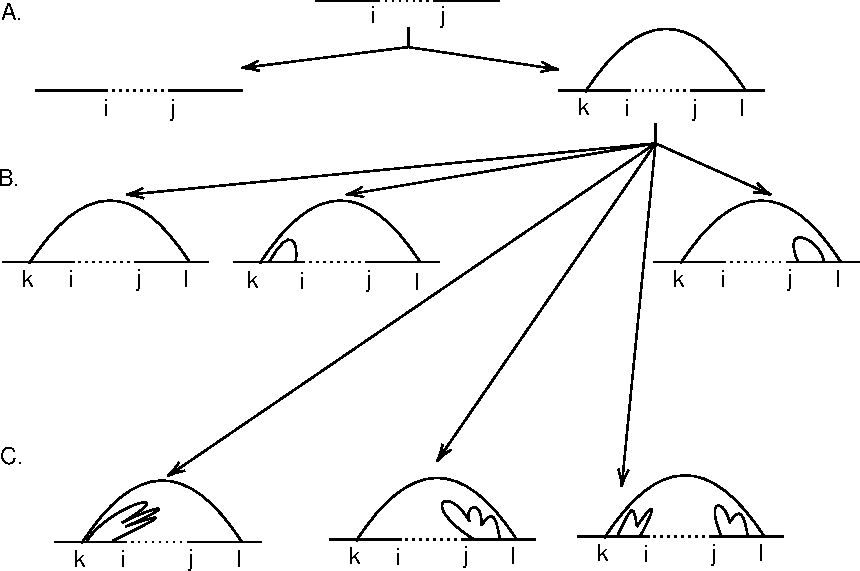
\includegraphics[width=1\textwidth]{chapters/Introduction/Figures/accs.pdf}
\caption[Decomposition of partition function to calculate unpairing probability of the region $(i,j)$ in a nucleotide sequence.]{\textbf{Decomposition of partition function to calculate unpairing probability of the region $[i,j]$ in a nucleotide sequence. (A)}  The interval [i,j] may either be enclosed by pair [k,l] (right) or may be open (left). \textbf{(B)} The enclosed pair may or may not contain an hairpin or \textbf{(C)} multiloops. The partition function $Z_{unpaired}$ is a sum of all these contributions.  Figure adapted from Bernhart \textit{et al.}, (2011)}%the List of Figures because of the *}
\label{fig:part_fun_decomp}
\end{figure}


% The exact equation to compute this probability and the accessibility in $\mathcal{O}(n^{3})$ time is given by Bernhart \textit{et al.}  with an algorithmic implementation in RNAplfold of ViennaRNA suite \cite{Lorenz2011-rg}. Accessibility prediction forms the basis of RNA:RNA interactions. 


\paragraph{RNA:RNA interactions} \label{subsec:rna_interac}
For two RNA molecules to interact and pair, most computational tools assume that this is  a two step process\textemdash unfolding of the RNA molecules at the target sites, followed by an actual interaction (hybridisation) \cite{Muckstein2006-ys}.
Thus, the total binding energy $\Delta G$ is the sum of the accessibility of the target site of the longer RNA molecule $\Delta G_{unpaired}$ and the subsequent interaction between the unfolded region of the interacting molecules $\Delta G_{int}$. $\Delta G_{unpaired}$ is computed by equation $1.8$, where as $\Delta G_{int}$ is computed through equation \ref{eqn:free_en} by replacing $Z$ with $Z_{int}$. For an interaction between nucleotides $[i, j]$ and $[i^*, j*]$ the partition function $Z_{int}$ is given by \cite{Muckstein2006-ys} (Figure \ref{fig:part_fun_interac}):





\begin{equation}
\begin{aligned}
    Z_{int} &= p_u[i,j] \sum_{i^*>j*} Z^I[i,j,i^*,j^*] \\
    where, \\
    Z^I[i,j,i^*,j^*] &= \sum_{\substack{i<k<j\\
    j*<k^*<i^*}} Z^1[i,k,i^*,k^*] e^{E_I(i,k,i^*,k^*)}
\end{aligned}
\end{equation}

with $E_I(i,k,i^*,k^*)$ as the free energy of the interior loop enclosed by $(i,k)$ and $(i^*,k^*)$ and $Z^1[i,k,i^*,k^*]$ contains at least one substructure between $(i,k)$ and $(i^*,k^*)$. 

\begin{wrapfigure}{r}{0.5\textwidth}
  \begin{center}
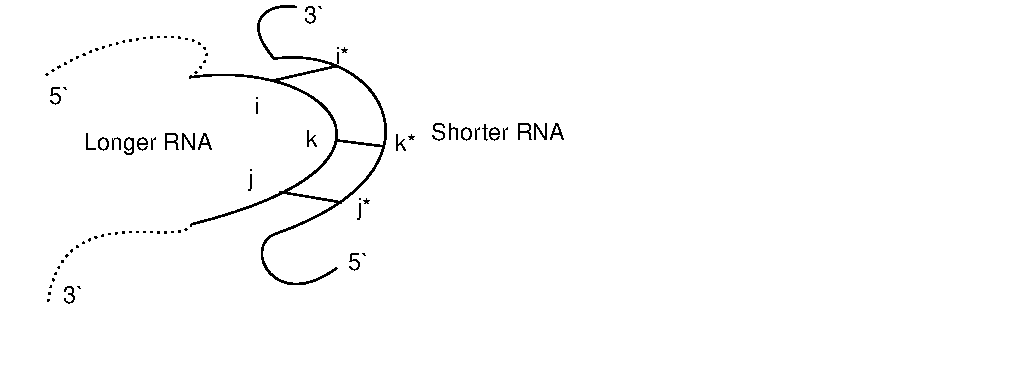
\includegraphics[width=0.7\textwidth]{chapters/Introduction/Figures/interac.pdf}
\caption[RNA:RNA interaction and notations used for partition function.]{\textbf{RNA:RNA interaction and notations used for partition function.} Full shape of longer RNA is not shown. The nucleotides between $[i,j]$ and $[i^*,j^*]$ may contain mismatches. Figure adapted from Muckstein \textit{et al.}, (2006). }%the List of Figures because of the *}
\label{fig:part_fun_interac}
  \end{center}
\end{wrapfigure}

The RNA:RNA interaction prediction mechanisms are still being actively refined because many RNA:RNA interactions have important regulatory functions. For example, in eukaryotes, microRNAs can reduce the levels of mRNAs by interacting with the $3^{\prime}$UTRs of the mRNA targets \cite{catalanotto2016microrna, valencia2006control}.










Apart from these general mRNA features which play a role in protein expression, several specific features also exist. For example: Cis-regulatory elements such as promoters and enhancers, interactions of mRNA with sRNA and miRNA as well as introns in $5^{\prime}$ UTR in eukaryotes. However, our discussion will be based around the general features only. 


A number of gene optimisation tools build a suitable cost or fitness function using a combination of these features. Typically, a genetic algorithm is then used to optimise the fitness. The synonymous mRNA sequence with the maximum fitness is regarded as the optimised mRNA sequence with optimal expression \cite{Villalobos2006-nx, Salis2009-dh, Raab2010-eg, Chung2012-zh, Terai2016-vp}. Despite being optimised on expression, the sequences may form aggregates, which cannot be used for further studies \cite{gustafsson2004codon, rosano2009rare}. This leads us to the discussion of optimising solubility. 


% Solubility
\subsection{Protein solubility}
% The Gibb's phase rule describes the state of a system at equilibrium and is given by 

% \begin{equation}
%     f + p = c + 2
% \end{equation}

% where $c$ is the number of components, $p$ is the number of phases and $f$ is the degree of freedom. For a two phase system (solid and liquid) at constant pressure and temperature, with two components (solute and solvent for example, protein and water), $f = 0$. This means the amount of protein in solution phase no longer depends upon the total amount of protein in the system and remains constant \cite{arakawa19853}. Thermodynamically, the chemical potential of protein in solid phase and liquid phase are now equal. The physical solubility, thus, can be defined as the concentration of protein in a saturated solution which is in equilibrium with the solid phase. Solubility has units of moles per liter ($m/L$) and often, for convenience, written in grams per liter ($g/L$). 


% This physical solubility of a protein depends on the experimental conditions such as temperature, pH, ionic concentration \cite{Kramer2012-wk}. This might lead to the variability of results across various experimental conditions. Hence, 
Solubility is defined as the proportion of the supernatant fraction, obtained after the centrifuging the the translation mixture, to the uncentrifuged total protein \cite{Niwa2009-ye}. It ranges from $0\%$ to $130\%$ with solubility less than $30\%$ categorised as aggregation-prone and greater than $70\%$ are highly soluble. Several \textit{intrinsic} features of the protein itself such as molecular weight, flexibility, hydrophobicity, isoelectric point and structural propensities are also known to influence solubility \cite{Wilkinson1991-zp, Chiti2003-zk, Tartaglia2004-wm, Diaz2010-md}. Sometimes these intrinsic features are modified by doing either mutagenesis or truncation, which might assist in improving solubility. Several solubility enhancing tags are also available for example, thioredoxin (TRX), maltose binding protein (MBP), small ubiquitin-related modifier (SUMO) and glutathione S-transferase (GST). Although, the exact mechanisms of how these tags work is still unclear, it is proposed that they might act like a chaperone and assist in correct folding of the target protein or add charges which decreases the overall aggregation propensity \cite{Costa2014-oe}.

\subsubsection{Intrinsic properties of a protein}
Intrinsic properties are derived from different properties of the residues inside the poly-peptide chain. The commonly used intrinsic properties of proteins are described below.

\paragraph{Hydrophobicity}
Water soluble proteins fold such that the hydrophilic parts are exposed and can form hydrogen bonds with the water molecules whereas the hydrophobic parts are buried in the core. This hydrophobic effect is thought to be responsible for protein solubility \cite{tanford1978hydrophobic}. Several scales have been proposed to measure the hydrophobicity of residues \cite{Kyte1982-qn, abraham1987extension, janin1979surface, rose1985hydrophobicity}. However, none of these scales can fully model the full range of behaviour of residues \cite{charton1982structural}. 


We will use Kyte-Doolittle's scale \cite{Kyte1982-qn} for representative purposes. In this scale, residues are given a hydropathy score such that positive scores represent hydrophobicity and negative score represent hydrophilicity. The magnitude of score represents the strength. For example: isoleucine (I) is given 4.5 and is the most hydrophobic residue, where as  arginine (R) is given -4.5 and is the most hydrophilic residue. Using these scores, a hydropathy plot for a given polypeptide can be drawn (Fig. \ref{fig:hydrophobicity_flexibility_plot}). Hydropathy plot can be used to examine the hydrophobicity of protein region of interest. Using hydrophobic effect, we can then infer whether the residue is buried or located on the surface. Furthermore, the overall hydrophobicity of the protein can be determined by averaging the hydropathy scores across the polypeptide chain to obtain the GRand AVerages of hydropathY (GRAVY) score.


\begin{figure}[htbp!]
\center
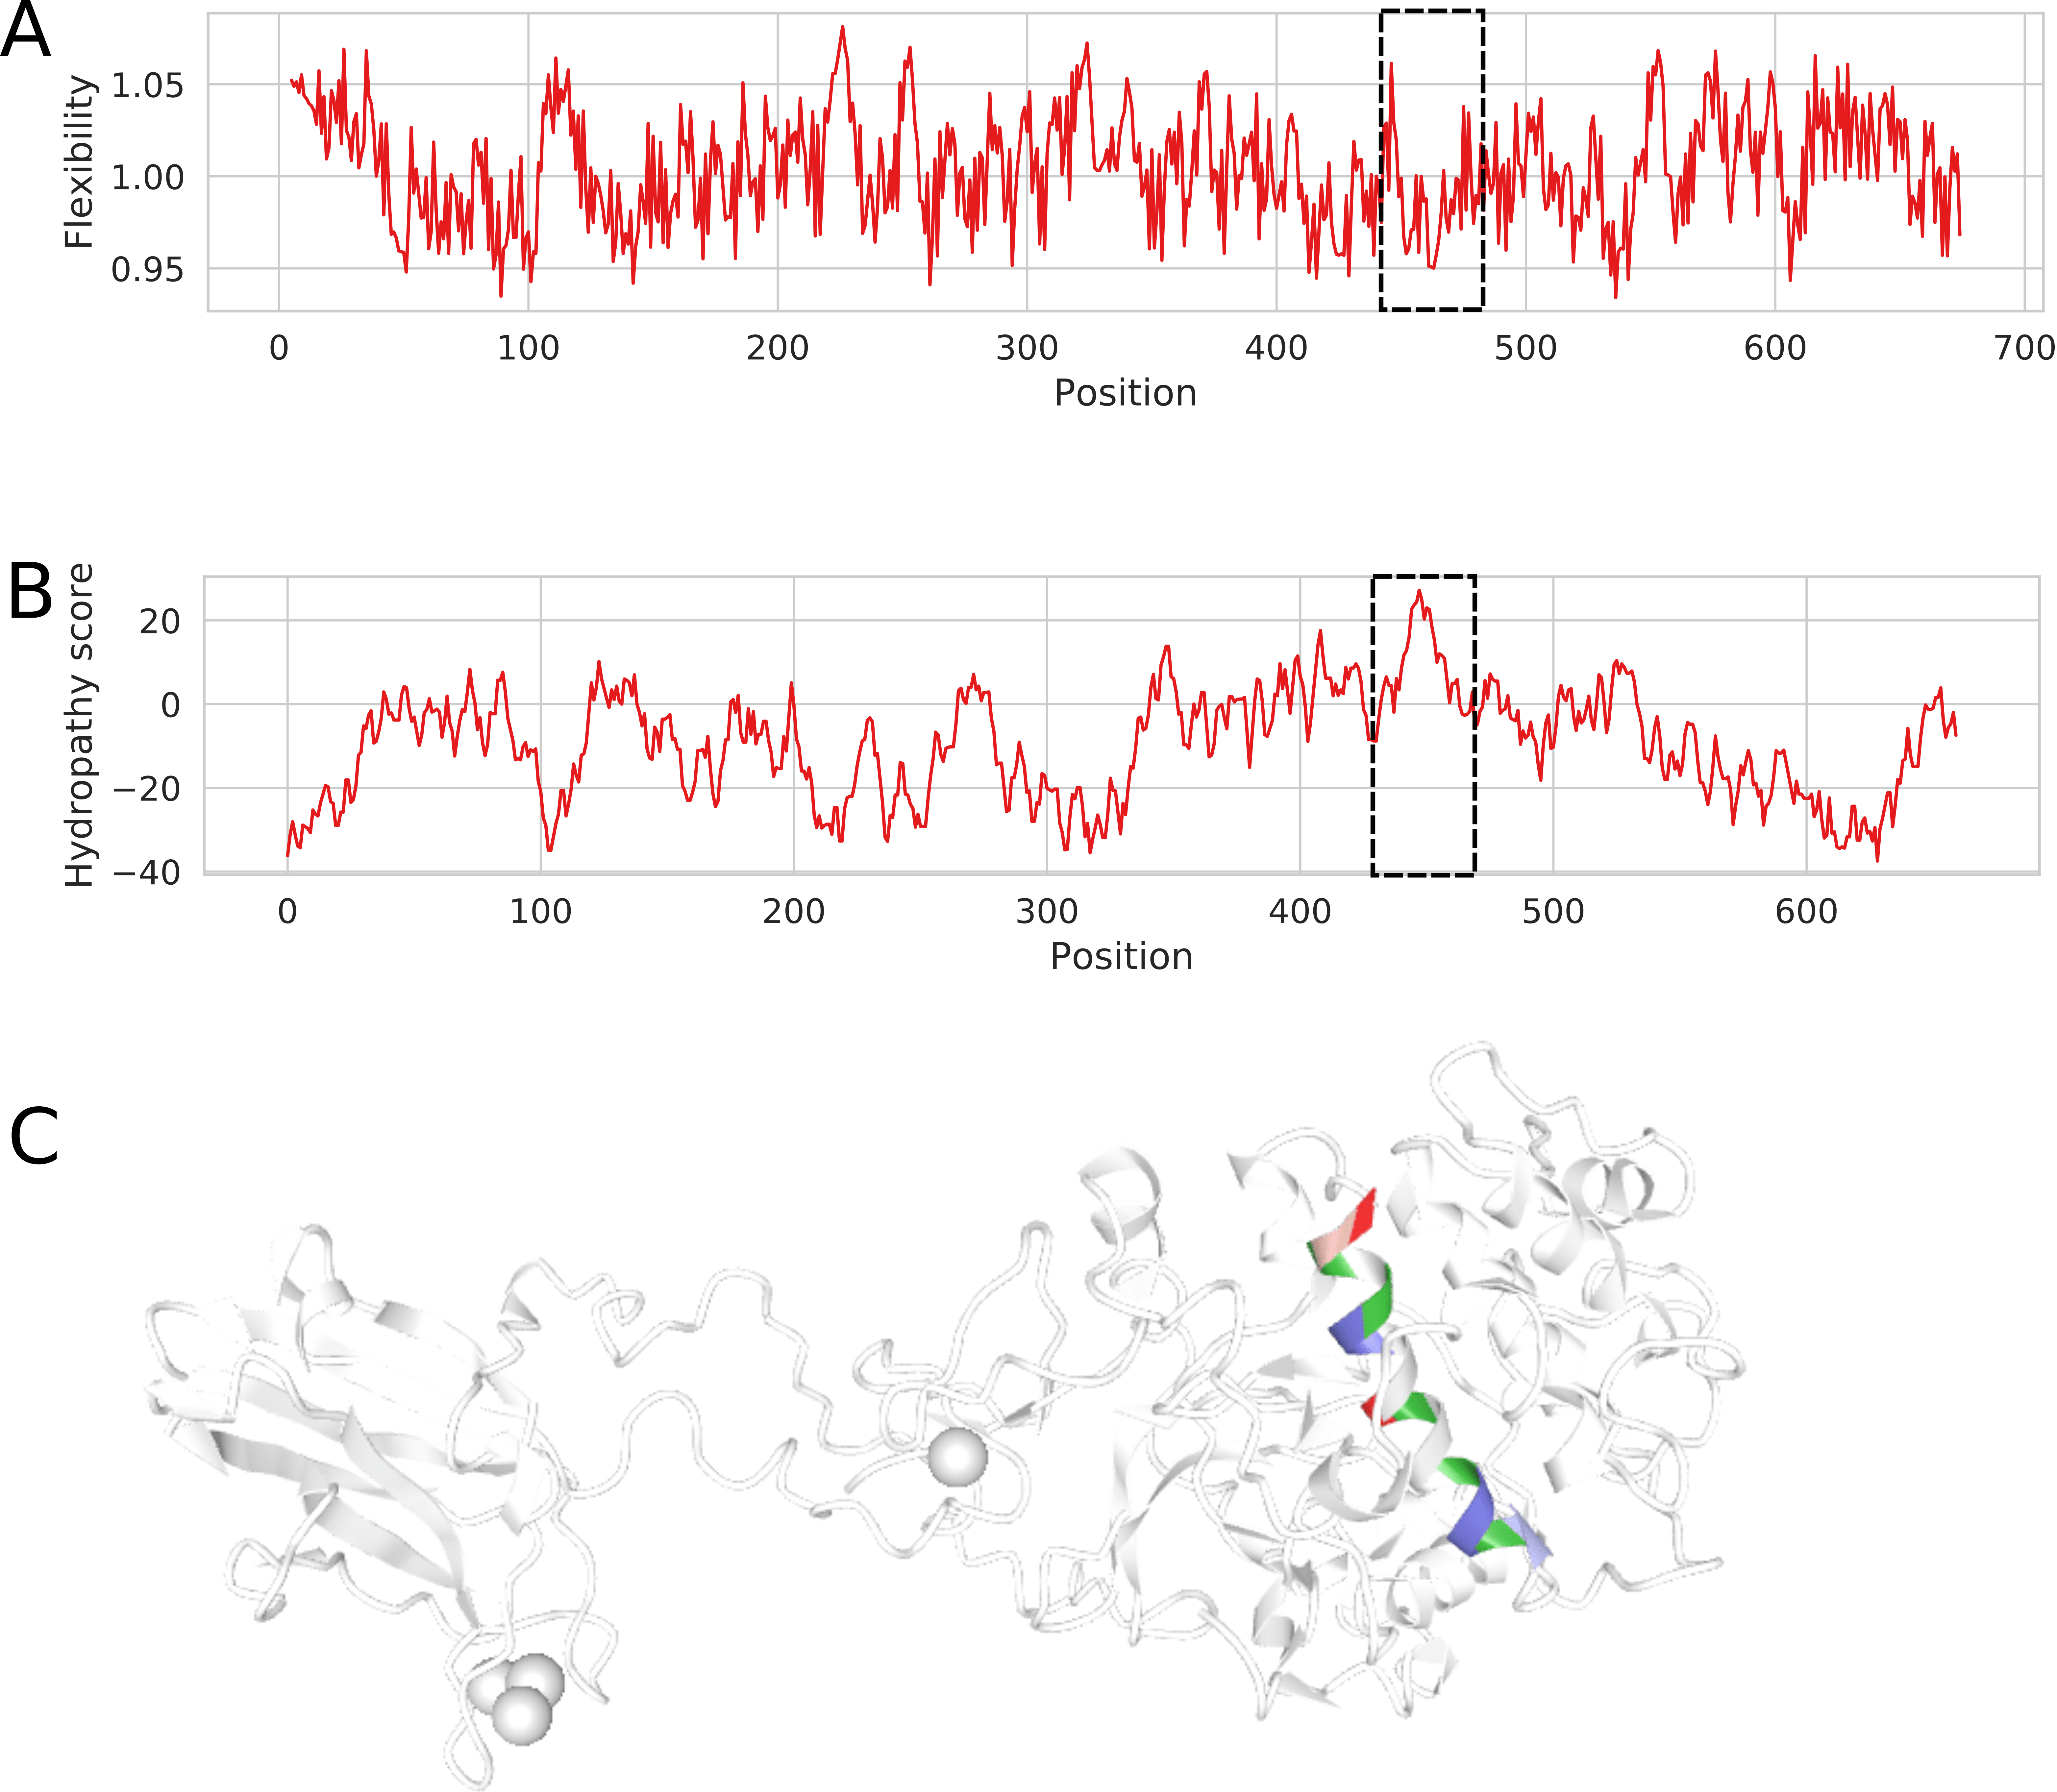
\includegraphics[width=1\textwidth]{chapters/Introduction/Figures/flex_and_hydrop.png}
\caption[Profiles of KPC1\_DROME (UniProtKB P05130).]{\textbf{Profiles of KPC1\_DROME (UniProtKB P05130)}. 
\textbf{(A)} Flexibility plot generated using normalised B-factors from Vihinen et al. (1994), with a sliding window of 9 residues. For these normalised B-factors, values greater than one are regarded to be flexible and values less than one are rigid. \textbf{(B)} Hydropathy plot generated using Kyte-Doolittle's hydrophobicity scale, with a sliding window of 19 residues. For illustration, the hydropathy and flexibility of residues at around position $440$ to $470$ (shown by dotted box) are positive and rigid. This indicates the presence of an alpha helix which is supported by the actual 3D structure \textbf{(C)}. The coloured helix is the region $440$ to $470$.  }%the List of Figures because of the *}
\label{fig:hydrophobicity_flexibility_plot}
\end{figure}


% \begin{figure}[htbp!]
% \center
% 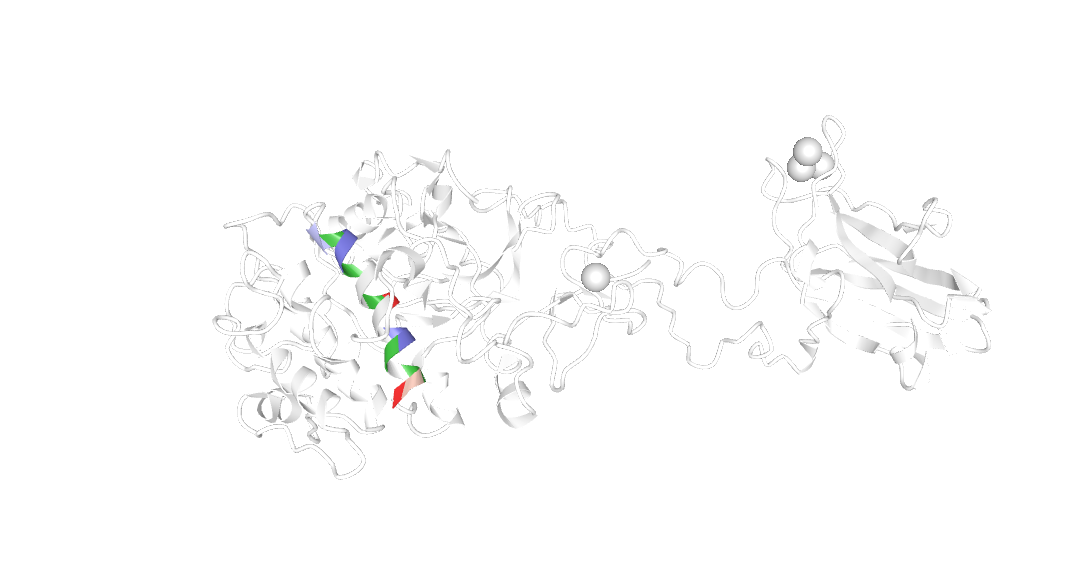
\includegraphics[width=1\textwidth]{chapters/Introduction/Figures/kpc1_drome.png}
% \caption{\textbf{3D structure of KPC1\_DROME (UniProtKB P05130)}. The highlighted helix runs from position $448$ to $467$. The presence of this helix can be inferred by the hydropathy plot (Fig \ref{fig:hydrophobicity_plot}) and the flexibility profile plot (Fig. \ref{fig:flexibility_plot}). }%the List of Figures because of the *}
% \label{fig:3dplot_kpc1_drome}
% \end{figure}


\paragraph{Isoelectric point}
The net charge of a protein at a given pH depends on acid dissociative constant (pKa) of ionisable groups such as amine and carboxyl group. At a certain pH, the amount of negative and positive charge are equal, resulting a zero net charge. This pH is called the isoelectric point (pI). The net charge is positive at pH below pI and negative at pH above pI \cite{shaw2001effect}. Since there are no net charges, the solubility of a protein is minimum at the isoelectric point.

\paragraph{Instability index}
Guruprasad et. al \cite{guruprasad1990correlation} found that the distribution of certain dipeptides on stable and unstable protein is different. Based on 12 unstable and 32 stable proteins, they assigned a weight called dipeptide instability weight value (DIWV) for all dipeptides. The instability index (II) is then given by equation \ref{eqn:instability_index}.

\begin{equation}
    II = \frac{10}{L}\sum_{i=1}^{L-1}DIWV(x_i y_{i+1})
    \label{eqn:instability_index}
\end{equation}

where $L$ is the length of the sequence and $x_i y_{i+1}$ is a dipeptide.

%%%http://pd.chem.ucl.ac.uk/pdnn/refine3/adps.htm
%%Biomolecular Crystallography: Principles, Practice, and Application : page 641

\paragraph{Flexibility}
Protein molecules are dynamic and are inherently flexible due to the motion of the constituent atoms \cite{vihinen1994accuracy, alvarez2014relationship, teilum2009functional}. The structural flexibility of a protein can be inferred by using B-factors \cite{vihinen1994accuracy, Karplus1985-ea, Smith2003-gb}.


The B-factor (Equation \ref{eqn:bfactor}) or temperature factor of the atoms in a crystalline structure is the measure of mean squared displacement vibration around their mean position $(u = \langle (x-x_0)^2 \rangle)$, where $x$ is the displacement of the atom from its mean position $x_0$. B-factor thus reflects the \textit{orderedness} of the crystal lattice and subsequent uncertainty in X-ray scattering structure determination \cite{Schlessinger2005-ps, Carugo2018-ka, Bramer2018-dh}. It has unit of $\AA^2$.


\begin{equation}
    B = 8\pi^2 u
    \label{eqn:bfactor}
\end{equation}

To understand the effect of the B-factor, we define a quantity $f$ called the atomic scattering factor as:

\begin{equation}
    f = \frac{amplitude\ of\ wave\ scattered\ by\ an\ atom}{amplitude\ of\ wave\ scattered\ by\ one\ electron}
\end{equation}

Atomic scattering factor after taking into account of the motion of atom becomes:

\begin{equation}
    f_B = f\cdot e^{-B(sin\ \theta /\lambda)^2}
\end{equation}

where $\theta$ is the Bragg angle and $\lambda$ is the wavelength of the wave. Thus, we see that B-factor attenuates the amplitude of wave scattered by an atom (Figure \ref{fig:bfactors} ).

% \begin{figure}[htbp!]
% \center
% 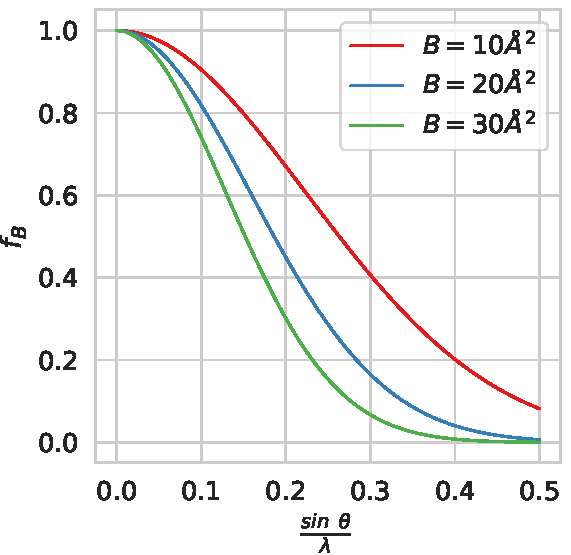
\includegraphics[width=0.5\textwidth]{chapters/Introduction/Figures/bfactors.pdf}
% \caption{\textbf{Attenuation of the incident waves due to increasing B-factor}. As B-factor increases, atomic scattering factor $(f)$ and consequently, the amplitude of wave scattered by an atom decreases rapidly.}%the List of Figures because of the *}
% \label{fig:bfactors}
% \end{figure}

Experimental B-factors for different residues in a protein sequence can be obtained the from Protein Data Bank (PDB). However, due to variation of structures, the B-factor of a given residue varies, even within the same polypeptide chain. For standardisation, the B-factor of residues within a chain are normalised using a z-score.

\begin{equation}
    B_{norm}^i =  \frac{B^i - \langle B\rangle}{\sigma}
\end{equation}

where, $B_{norm}^i$ is the normalised B-factor of residue $i$, $\langle B\rangle$ is the mean and $\sigma$ is the standard deviation of all B-factors across the chain.

\begin{wrapfigure}{r}{0.5\textwidth}
  \begin{center}
    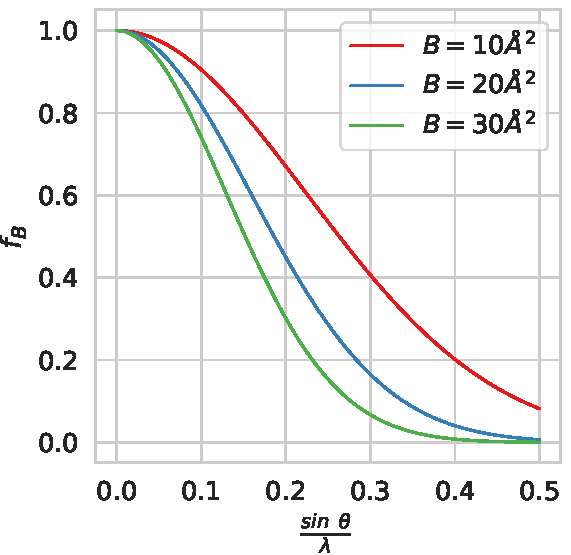
\includegraphics[width=0.45\textwidth]{chapters/Introduction/Figures/bfactors.pdf}
    \caption[Attenuation of the incident waves due to increasing B-factor.]{\textbf{Attenuation of the incident waves due to increasing B-factor.} As B-factor increases, atomic scattering factor $(f)$ and consequently, the amplitude of wave scattered by an atom decreases rapidly.}%the List of Figures because of the *}
    \label{fig:bfactors}
  \end{center}
\end{wrapfigure}


A number of high resolution structures are sampled from database and $B_{norm}^i$ is calculated for each residue on each protein. The mean of $B_{norm}^i$ across the sampled structures is the final normalised B-factor \cite{Schlessinger2005-ps, Smith2003-gb, Karplus1985-ea, vihinen1994accuracy}. 


The structural flexibility of protein can either be determined by using these normalised B-factors from experiments or by directly computing atomic displacements form molecular dynamics simulations (MDS) 
\cite{dong2018structural, kufareva2011methods}. Root mean square fluctuations and radius of gyration from MDS are useful in examining the flexibility. The profile plot (Fig. \ref{fig:hydrophobicity_flexibility_plot}) can be used to visualise and infer the local flexibility and dynamics of the protein structure. Since structural flexibility is inherently related to the protein dynamics, it is thought to influence several properties such as conformal variations, functions, thermal stability, ligand binding and disordered regions  \cite{Vihinen1987-jo, Teague2003-vq, Ma2005-cr, Yuan2005-gl, Yin2011-su, amaral2017protein}. Although the relationship of flexibility with solubility has been noted previously \cite{Tsumoto2003-qp}, it has been overlooked. 


% \begin{figure}[htbp!]
% \center
% 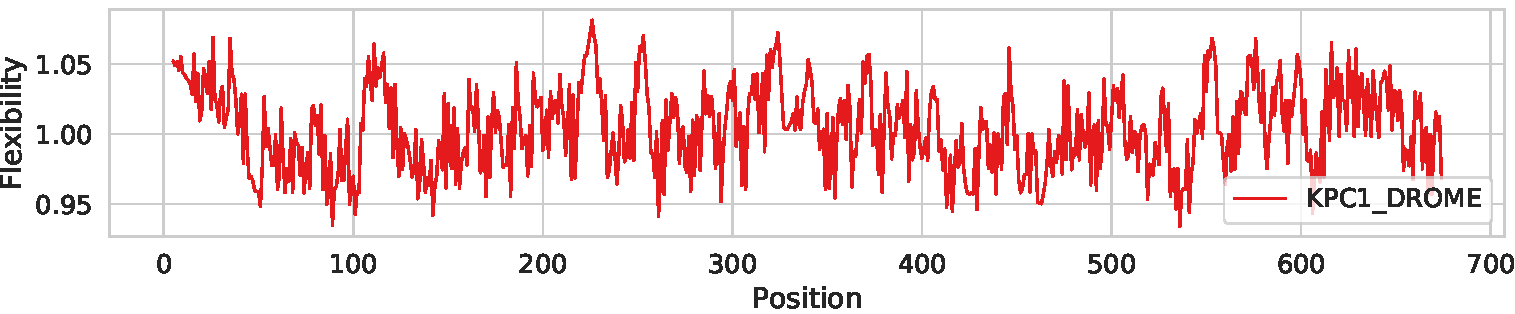
\includegraphics[width=1\textwidth]{chapters/Introduction/Figures/flexibility.pdf}
% \caption{\textbf{Flexibility profile of KPC1\_DROME (UniProtKB P05130)}. Plot was generated using normalised B-factors from Vihinen et al. (1994), with a sliding window of 9 residues. For these normalised B-factors, values greater than one are regarded to be flexible and values less than one are rigid. For illustration purposes, the residues at around position $440$ to $470$ are rigid, suggesting that there might be some structures. This is also supported by the hydropathy plot (Fig. \ref{fig:hydrophobicity_plot}) and the actual 3D structure (Fig. \ref{fig:3dplot_kpc1_drome}).}%the List of Figures because of the *}
% \label{fig:flexibility_plot}
% \end{figure}


Beside these features, amino acids also tend to have different structural propensities which is also thought to influence protein solubility \cite{Idicula-Thomas2005-qw, Huang2012-ft}.


Many solubility prediction tools have been developed around these features using statistical models (e.g., linear and logistic regressions) and machine learning models (e.g., support vector machines and neural networks) \cite{Hirose2013-nq, Habibi2014-jq, Hebditch2017-bg, Sormanni2017-lo, Heckmann2018-wb, Wu2019-nz, Yang2019-kd}. Newer tools such as SOLart also employ 3D structural information for a precise estimation of solvent accessibility, which makes the prediction more accurate \cite{hou2020solart}. Despite a higher prediction accuracy, the usability of these structure based tools might be limited due to the lack of 3D structure information of many proteins of interest.





% Signal peptides
\section{Signal Peptide}
Secretory proteins such as hormones and toxins are some of the commercially important use cases of recombinant protein expression. These secretory proteins are often enriched with a short hydrophobic peptide at the N-terminal (Figure \ref{fig:signal_peptides}). This is called signal peptide (SP). Signal peptides are recognised by a protein complex called the signal recognition particle (SRP). SRP carries the signal peptide to the endoplasmic reticulum (ER) lumen, where post translation modification happens and the newly synthesised protein is secreted out.  Despite having no consensus, SP have a tripartite structure as N-region, H-region and C-region \cite{Von_Heijne1985-qv} (Figure \ref{fig:signal_peptide_structure}). 

\begin{figure}[htbp!]
\center
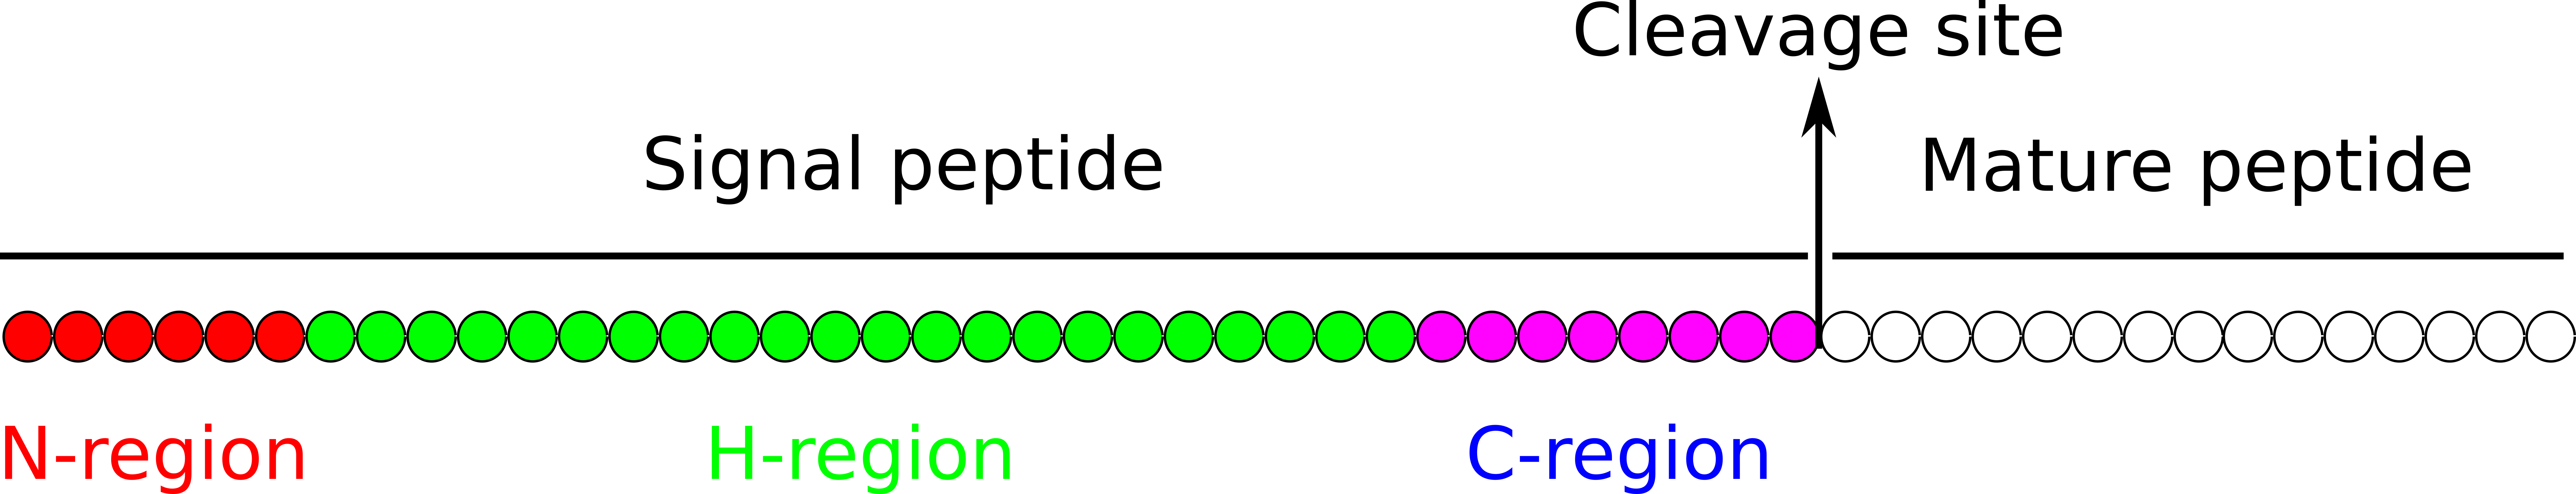
\includegraphics[width=1\textwidth]{chapters/Introduction/SignalPeptide/Figures/signal_peptide.png}
\caption[Tripartite structure of a signal peptide.]{\textbf{Tripartite structure of a signal peptide.} N, H and C domains in a signal peptide. C domain also contains a cleavage site from which mature peptide is cleaved off after reaching the endoplasmic lumen. Sequence logo (bottom) shows an enrichment of Leucine (L) at the H-region.}
\label{fig:signal_peptide_structure}
\end{figure}


\begin{wrapfigure}{r}{0.5\textwidth}
  \begin{center}
    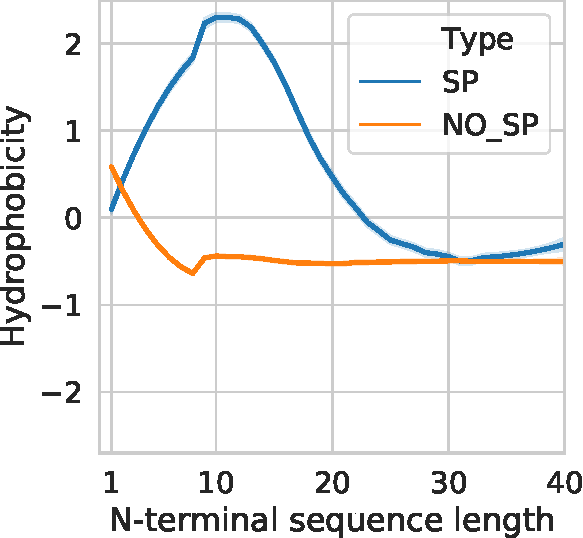
\includegraphics[width=0.45\textwidth]{chapters/Introduction/SignalPeptide/Figures/sp_nosp_lineplot.pdf}
    \caption[Signal peptides are highly hydrophobic at the N-terminal.]{\textbf{Signal peptides are highly hydrophobic at the N-terminal.} Savitzky–Golay filtering is applied to the hydrophobicity. SP (N=2,609) and NO\_SP (N=14,655) sequences from SignalP 5.0 dataset (Armenteros \textit{et al.} (2019)). SP, Signal Peptide; NO\_SP, Not a SP.}%the List of Figures because of the *}
    \label{fig:signal_peptides}
  \end{center}
\end{wrapfigure}
The N-region usually consists of 2-5 charged residues, whereas the H-region is highly hydrophobic and forms an alpha helix. The C-region consists of small polar uncharged residues which often form a $\beta$-sheet structure. This topology is thought to help binding with signal peptidase and cleave off the signal peptide at the cleavage site. 

% Translation is temporarily paused when signal recognition particle (SRP) binds to the SP. SRP then carries the ribosome/mRNA complex towards the translocon of endoplasmic recticulum (ER). Signal peptide is then detached from the mature peptide and possibly digested by signal peptidase. Translation resumes, pushing the nascent polypetide inside the ER lumen, where post translation modification happens and the newly synthesised protein is secreted out. 

The use of signal peptides in recombinant expression can lead to a high yield. As an added benefit, the proteins are often closer to the native activity because proper folding can happen inside the ER \cite{Futatsumori-Sugai2010-iu, Karyolaimos2019-ip}. 



% Optimisation methods
\section{Mathematical optimisation}
Optimisation is a way to find out the best solution to the problem. The starting point for optimisation is to define an objective function or the cost function. For an objective function $f: A \rightarrow  \mathbb{R}$, the goal of optimisation is to find $x_0 \in A$ such that $f(x_0) \leq f(x)$ $\forall\ x \in A$. If the objective function is differentiable, then we can use the gradient information to reach the optimal point. Non differentiable functions are usually optimised by heuristic optimisation methods. Heuristic methods often provide a near optimal solution even if the search space is large. The following optimisation methods are used in this study.


\subsection{Simulated annealing}
\label{subsection:sim_anneal}
Simulated annealing is a heuristic optimisation technique inspired by the way metals cool and anneal. More precisely, it is based on the thermodynamics of a system undergoing a slow cooling so that the atoms have sufficient time to redistribute to form a crystalline structure\textemdash a state of minimum energy  \cite{Kirkpatrick1983-hh, Ingber2000-aw, Keith2002-jx, Brownlee2011-bk, presse1988numerical}. Simulated annealing algorithm is often used to solve combinatorial optimisation problems in bioinfomatics and other sciences. It has been used to align and predict non-coding RNAs from multiple sequences \cite{Lindgreen2007-jy}, to find consensus sequences \cite{Keith2002-jx} and optimise the ribosome binding sites \cite{Salis2009-dh} and mRNA folding using minimum free energy models \cite{Gaspar2013-bg}.

Let $p_i$ is the probability that a system is in certain state $i$ with energy $\epsilon_i$. Then entropy of the system is defined as:
\begin{equation}
    S = -k_B\sum_{i} p_i \ln(p_i)
    \label{eqn:entropy}
\end{equation}
where $k_B$ is the Boltzmann's constant. For any system, the second law of thermodynamics states that the entropy is maximised as the system evolves towards a  thermodynamic equilibrium. Hence, to know the behaviour of the system, Equation \ref{eqn:entropy} needs to be maximised under these two constrains:
\begin{equation}
    \begin{split}
        1)\ \sum_j p_j &= 1 \\
        2)\ \sum_j p_j \epsilon_j &= E
    \end{split}
\end{equation}
The first condition simply means that sum of all probabilities should be unity while the second condition implies the total energy of the system is constant. Using Lagrange multipliers,  
\begin{equation}
    S = -k_B\sum_j p_j \ln(p_j) - \lambda [\sum_j p_j -1 ] - \beta[\sum_j p_j \epsilon_j - E]
    \label{eqn:lagrange_mult}
\end{equation}
Setting the first derivative of Equation \ref{eqn:lagrange_mult} to zero, we obtain:
\begin{equation}
    p_i = e^{1-\lambda}.e^{-\beta \epsilon_i}
    \label{eqn:prob_aft_max}
\end{equation}
$\beta$, also known as thermodynamic beta, can be shown to be equal to $1/k_B T$, where $T$ is the absolute temperature. $\lambda$ is chosen to normalise the probability $p_i$ in Equation \ref{eqn:prob_aft_max}. We thus arrive at the Boltzmann's probability distribution:
\begin{equation}
    p_i = \frac{1}{Z} e^{-\beta \epsilon_i}
    \label{eqn:prob_boltzmann}
\end{equation}
where $Z$ is the partition function. For a system in thermal equilibrium at temperature $T$, Equation \ref{eqn:prob_boltzmann} gives us a set of probability mass functions for all different energy states $\epsilon_i$. An interesting implication of the Boltzmann's distribution is that even at low temperature, there is a non zero probability of system being at high energy.  


Mathematical way to reach the minima of the Boltzmann's distribution is by using a Markov chain sampling while simultaneously decreasing the temperature. The decreasing temperature is simulated by applying a cooling schedule, which could be exponentially decreasing \cite{Kirkpatrick1983-hh}. Markov chain sampling can be done by using Metropolis-Hastings algorithm or perhaps Gibb's sampling, although it is less commonly used  \cite{Keith2002-jx}. In Metropolis-Hastings algorithm, a \textit{bad} move (uphill) $E_2$ from initial state $E_1$ such that $E_2 > E_1$, is accepted if $R(0,1) \geq p_2/p_1$, where $R(0,1)$ is a uniformly random number between $0$ and $1$ \cite{hastings1970monte}. Unlike gradient descent, where only \textit{good} moves (downhill) ($E_2 < E_1)$ are accepted, this algorithm thus, can move both uphill and downhill without getting trapped in local minima. The probability of system moving uphill, however, decreases with decrease in temperature \cite{presse1988numerical}. 


%‘bad’ move
A use case of simulated annealing on a Rastrigin function (Figure \ref{fig:rastrigin}) is shown in Figure \ref{fig:sim_anneal}. 

\begin{figure}[H]
\center
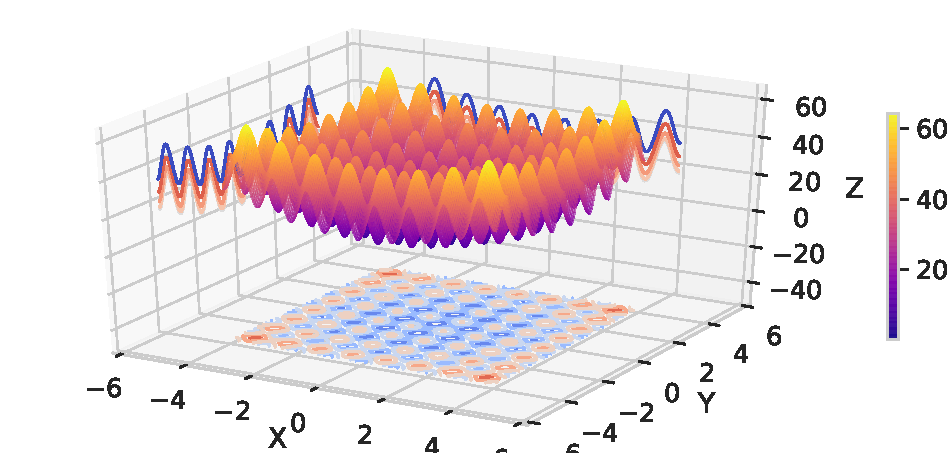
\includegraphics[width=1\textwidth]{chapters/Introduction/Figures/rastrigin.pdf}
\caption[Two dimensional Rastrigin function.]{\textbf{Two dimensional Rastrigin function.} Rastrigin function is frequently used as a test function in optimisation problems because of a large number of local minima. The global minima is at $(0, 0)$ where the value of function is $0$.}%the List of Figures because of the *}
\label{fig:rastrigin}
\end{figure}


\begin{figure}[H]
\center
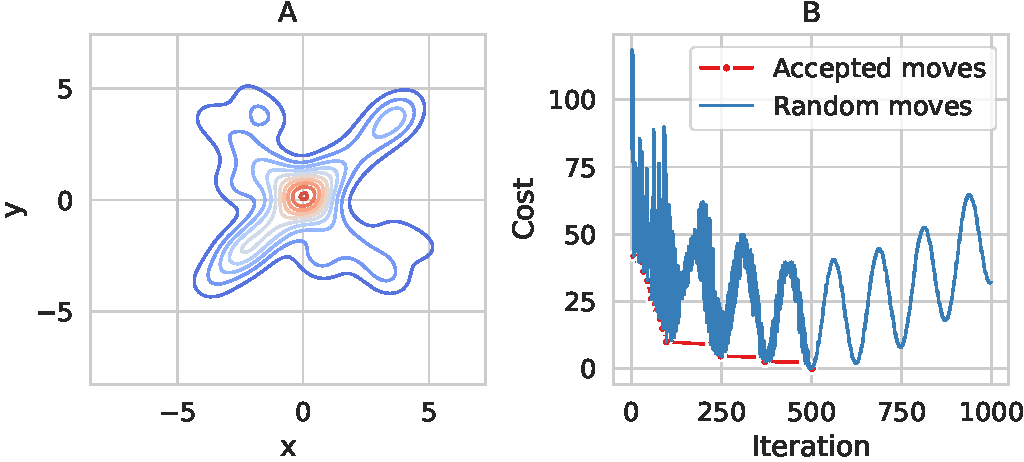
\includegraphics[width=1\textwidth]{chapters/Introduction/Figures/simulated_annealing.pdf}
\caption[Simulated annealing on a two dimensional Rastrigin function.]{\textbf{Simulated annealing on a two dimensional Rastrigin function.} This simulation was run for $1,000$ iterations with an initial temperature of $1$. The minimum found was at $(0.006, -0.013)$, where the value of function was $0.04$.  \textbf{(A)} Kernel density estimate of the moves during simulated annealing shows that they converge near the true minimum $(0, 0)$. \textbf{(B)} The accepted costs are usually immune to the traps of local minima. The algorithm converted at $502^{nd}$ iteration, where the accepted cost is $0.04$. This is close to the global minima $0$. }%the List of Figures because of the *}
\label{fig:sim_anneal}
\end{figure}


\subsection{Nelder-Mead method}
The Nelder-Mead method is another type of derivative-free, heuristic optimisation technique \cite{Nelder1965-zb}. The method, however, requires the objective function to be evaluated at different points hence can also be categorised as a \textit{direct search} method. Direct search methods usually employ a non-degenerate simplex at each step \cite{lagarias1998convergence}. 

% \footnote{Simplex in $n$ dimensions is a convex-hull of $n+1$ vertices and can be understood as a generalisation of triangles. By non-degenerate, we mean the volume of the simplex is non zero.}

For an $n$ dimensional function $f(x)$, initialisation is done by choosing $n+1$ points $(x_i, 1\leq i \leq n+1)$ which form a simplex. These points are ordered such that $f(x_1) \leq f(x_2) \leq ... f(x_{n+1})$. Since the goal is to minimise $f(x)$, in this case $x_{n+1}$ is the worst point and $x_1$ is the best. The worst point is then reflected along the centroid of the simplex to give a new vertex $x_r$ such that the volume is preserved and the non-degeneracy is maintained \cite{presse1988numerical}. Three cases may happen:

\begin{itemize}
  \item $f(x) \leq f(x_r) \leq f(x_{n+1})$
  
  In this case, the new move is neither good nor bad. $x_r$ replaces some older point $x_o$ where $f(x) \leq f(x_o) \leq f(x_{n+1})$.
  
  \item $f(x) \leq f(x_{n+1}) \leq f(x_r) $
  
  In this case, the new move is worst. The simplex is contracted by decreasing $x_{n+1}$ to $x_c$. If $x_c < Min(f(x_{n+1}), f(x_r))$, $x_{n+1}$ is replaced by $x_c$. Else, contraction is repeated.
  
  \item $f(x_r) \leq f(x_1) \leq f(x_{n+1}) $
  
  In this case, the new move is good. $x_r$ replaces the older best point $x_1$. 
\end{itemize}

The ordering of points and reflection are repeated, until the change in the value of the function at the best point falls below a preset tolerance. This method tends to get stuck at local minima (Figure \ref{fig:nelder-mead} A, B), because whenever it encounters one, the algorithm contracts the simplex rather than exploring the surrounding. However for functions with a few or no local minima, for example, Rosenbrock function (Fig. \ref{fig:rosen}), if the starting point is good, this algorithm is very efficient in finding the minima (which is often global) (Figure \ref{fig:nelder-mead} C, D).


\begin{figure}[H]
\center
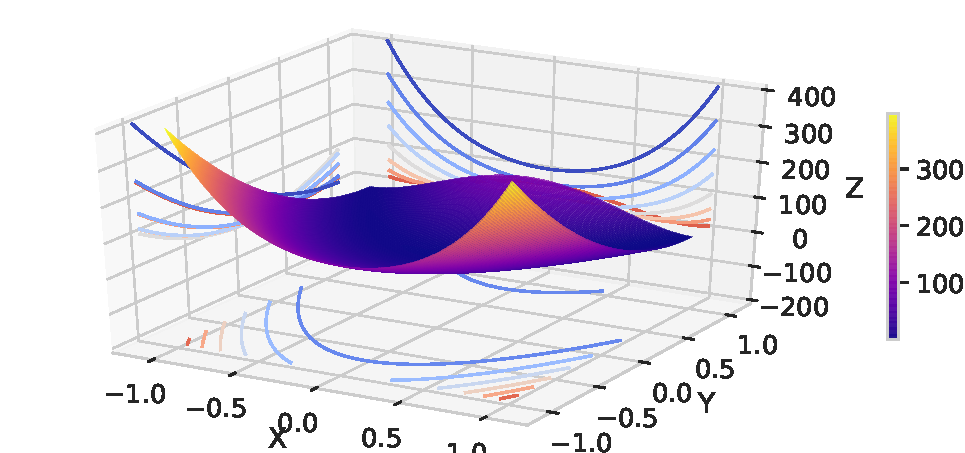
\includegraphics[width=0.75\textwidth]{chapters/Introduction/Figures/rosen.pdf}
\caption[Two dimensional Rosenbrock function.]{\textbf{Two dimensional Rosenbrock function.} Rosebrock function has a characteristic valley where the global minimum lies. The global minima is at $(1, 1)$ where the value of function is $0$.}%the List of Figures because of the *}
\label{fig:rosen}
\end{figure}

\begin{figure}[H]
\center
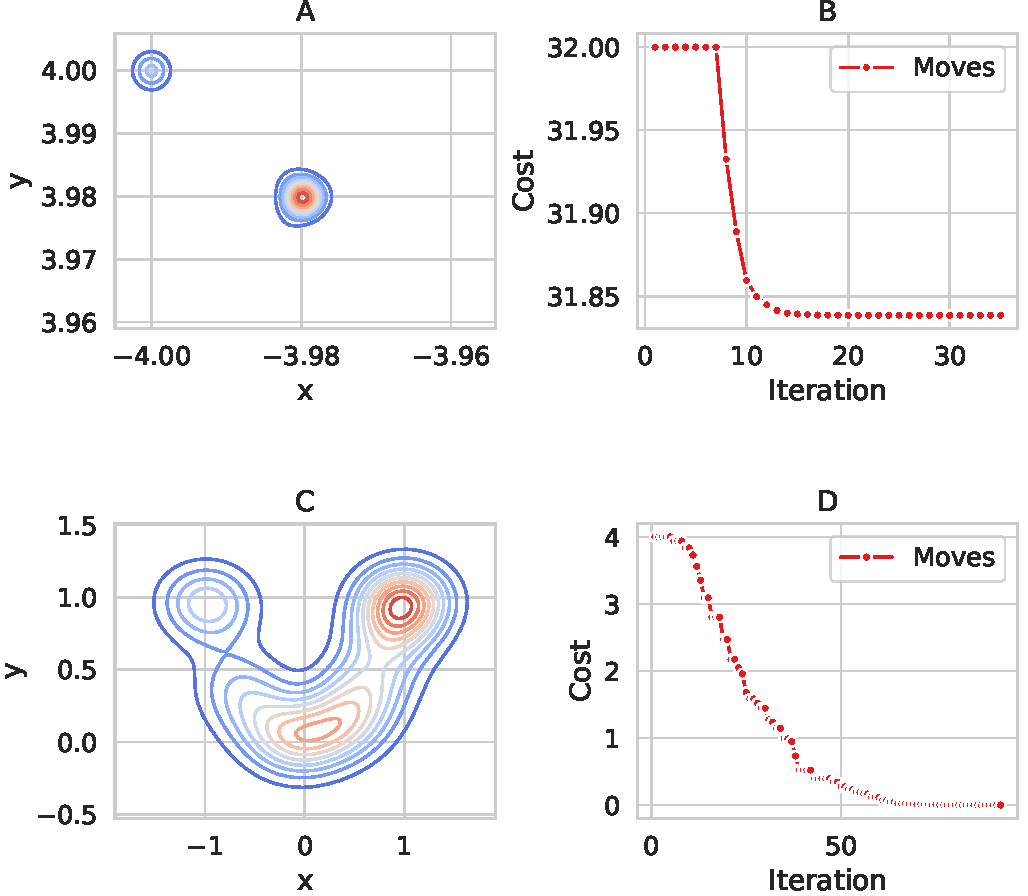
\includegraphics[width=0.75\textwidth]{chapters/Introduction/Figures/Nelder-Mead.pdf}
\caption[Although the Nelder-Mead method tends to get stuck on local minima, a good initial point can result in a global optimum.]{\textbf{Although the Nelder-Mead method tends to get stuck on local minima, a good initial point can result in a global optimum.} \textbf{(A)} Nelder-Mead method applied on a Rastrigin function. Kernel density estimate of the moves shows that the algorithm gets stuck at a local minima $(-3.98, 3.98)$. \textbf{(B)} The algorithm terminated after $35$ iterations where the minimum was found to be $3.36$, which is a local minimum. \textbf{(C)} Nelder-Mead method applied on a Rosenbrock function with $(-2,2)$ as the starting point. Kernel density estimate of the moves shows that the algorithm moves around the valley and terminates at $(1.0001, 1.0002)$ close to the global minima. \textbf{(D)} The algorithm terminated after $92$ iterations where the minimum was found to be $3.36 \times 10^{-8}$.}%the List of Figures because of the *}
\label{fig:nelder-mead}
\end{figure}

% Classifier
\section{Classifiers}
Classifiers are functions which map the input vector to some specific category. In the context of machine learning, we usually use a set of labelled data (known as training data) to fit a classifier. This fitted classifier, also known as model, can then be used to do predictions on unknown data. Many types of classifiers exist such as linear classifiers, support vector machines, decision trees and neural networks (Figure \ref{fig:classifier_comparision}). One special classifier built from an ensemble of decision trees called the Random forest classifier is used in this work. 

\subsection{Random forest}
A random forest is a classifier consisting of a collection of tree structured classifiers $\{h(x, \Theta_k), k=1, ...\}$ where the  $\{\Theta_k\}$ are independent, identically distributed random vectors and each tree casts a unit vote for the most popular class at input {x} \cite{breiman2001random}. For a given data, a number of decision trees $B$ are constructed using bootstrapping. Every time a new split is done, a subset $m$ of total vectors (features) $f$ is used, such that $m < f$. If $m = f$, this procedure is called bagging. In practise, usually, $m \approx \sqrt{f}$. Surprisingly, the number of trees, $B$, is not critical and setting this to a very high value will not lead to overfitting, which can be shown to be a consequence of strong law of large numbers \cite{james2013introductiontostatlearning, breiman2001random}. This also makes random forests more robust to noise and outliers than other classifiers. 

Typically, each bagged tree uses around two-third of training points. Out-of-bag (OOB) estimates can be computed by preforming predictions on the remaining one-third points. OOB errors reflect the generalisability of the model. For each feature, we can also compute the total reduction of Gini index by that feature at each tree split, where Gini index is defined by: 
\begin{equation*}
    G = \sum_{k=1}^{K}(p_{mk}(1-p_{mk}))
\end{equation*}
and is a measure of variance across $K$ classes for the proportion of training observations, $p_{mk}$, in the $m^{th}$ region that are from the $k^{th}$ class. This gives us the feature importance, sometimes called the Gini importance. However, it should be noted that $m$ features used for each split are actually random and is not based on feature importance at all. This seemingly deceptive strategy forces all the subsequent trees to not use the same strongest predictor, thus forcing a decorrelation among the trees. This makes the outputs less variable and more reliable.

\begin{figure}[!hbtp]
\centerline{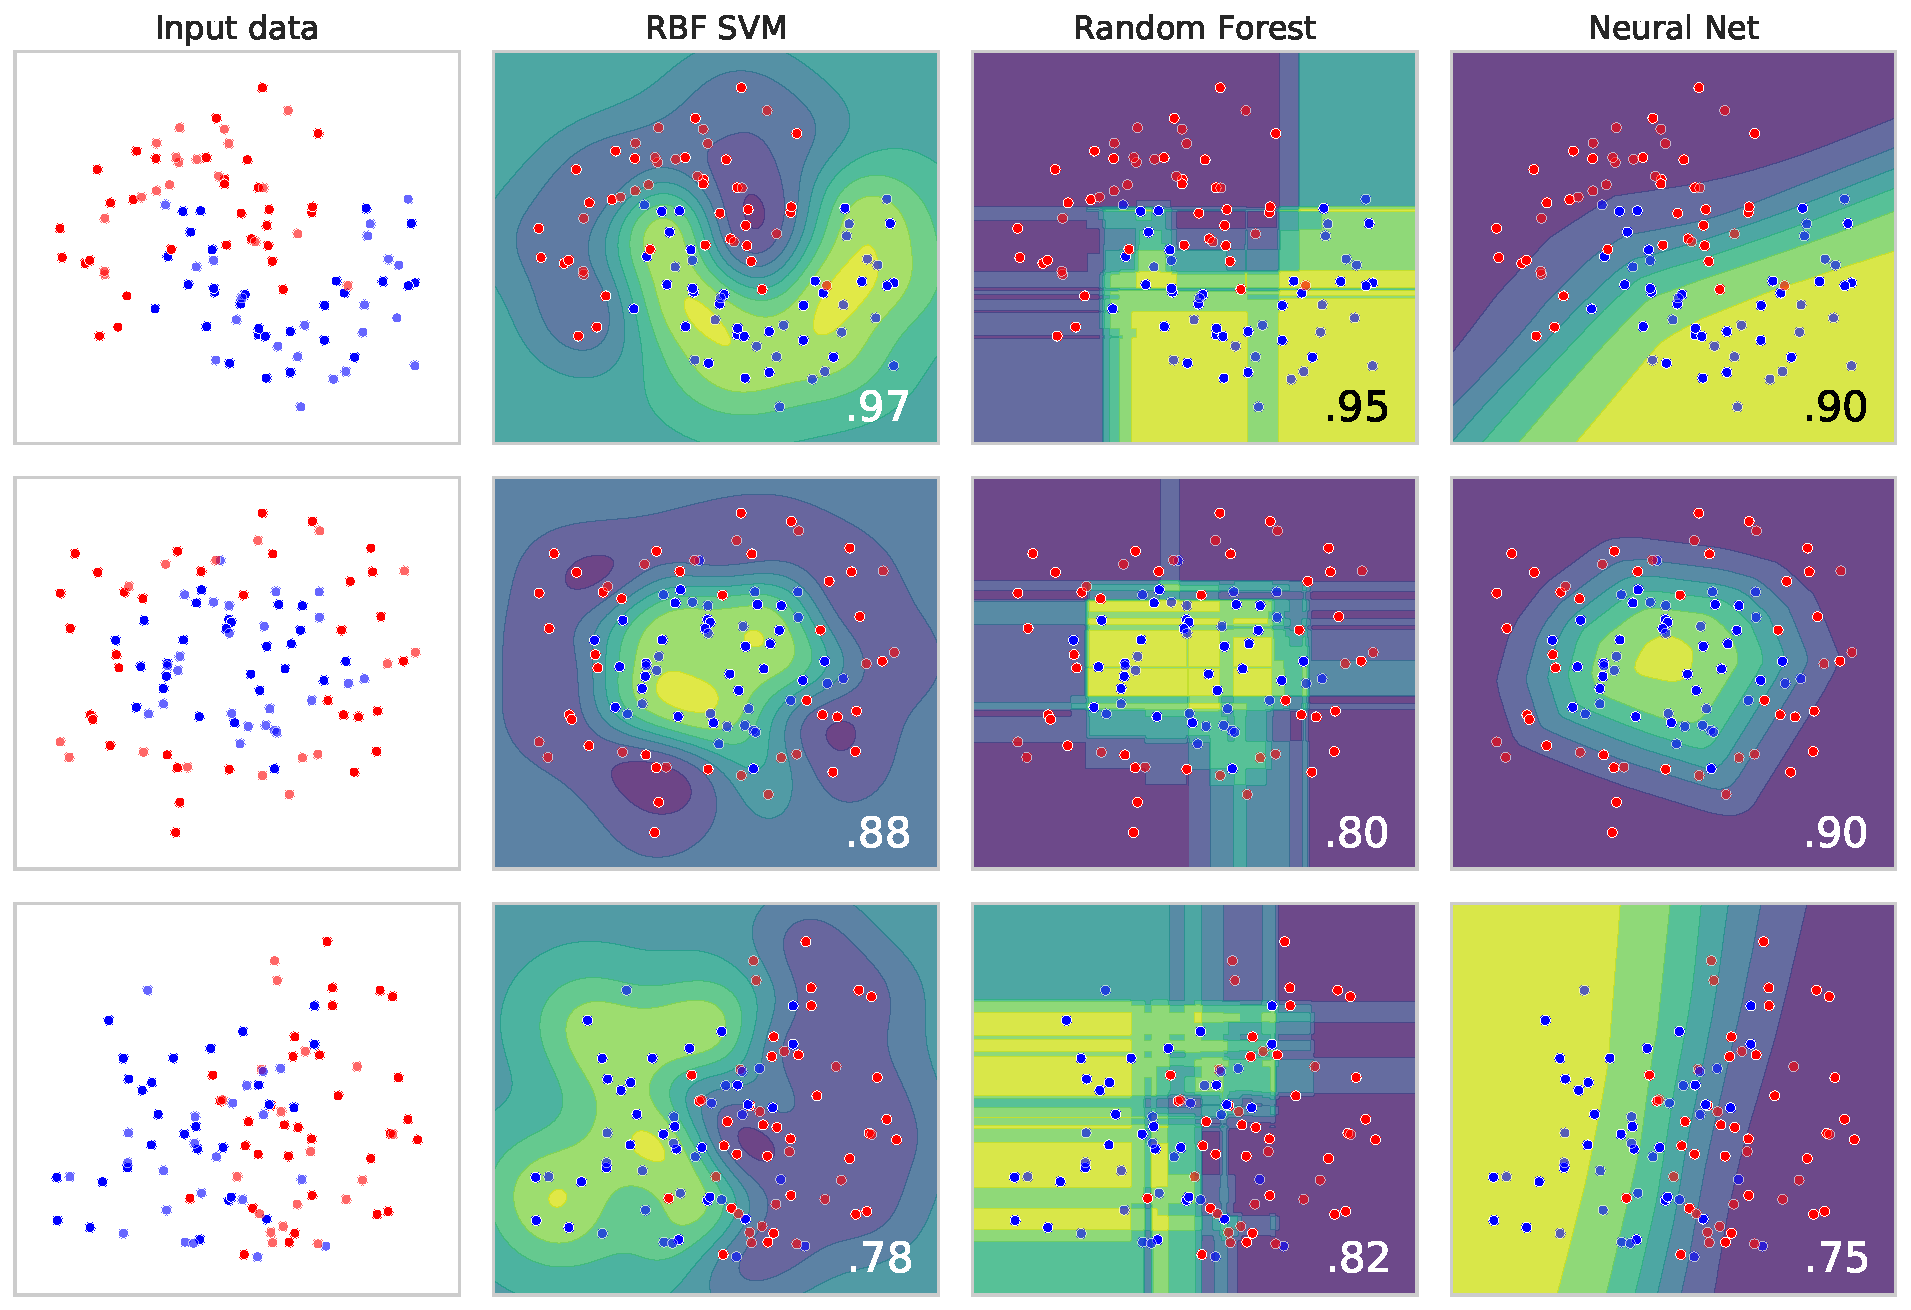
\includegraphics[width=1\textwidth]{chapters/Introduction/Figures/classifier_comparision.pdf}}
\caption[Comparison between some of the commonly used classifiers.]{{\bf Comparison between the some of the commonly used classifiers.} Three commonly used classifiers\textemdash SVM with RBF kernel, Random forest and a simple neural network (multi-layered perceptron) on three synthetic datasets as input. The input data is a binary data coloured as red and blue. The decision boundary is shown as contours and the accuracy of each classifier is shown on bottom right. Adapted from https://scikit-learn.org/stable/auto\_examples/classification/plot\_classifier\_comparison.html. SVM, Support Vector Machine; RBF, Radial Basis Function.}\label{fig:classifier_comparision}
\end{figure}






